Through the earlier experimentations with the graph generations based on specific properties, improvements have been made. This includes normalisation of the values into the range of 0-10 rather than using a scale factor. Which ensures that all the graphs will be similarly shaped and have the same axis size for an easier visual comparison. Also I've included page rank as well as the other graph properties used before. Finally the datasets I will use will be generated through my program by an input of text. Afterwards will be converted into graphs where the words represent the vertices and the edges are directed to the next word in the order of the text. A factor that affected the dataset was the punctuation so to achieve congruent data, the punctuation are stripped unless they are sentence enders such as full stops, question marks, exclamation marks etc. 

Therefore, the graph we experiment on are directed graphs generated from various language families.

\section{Linguistics}
Modern languages are decendantrs of ancestral langauges thoruhg eveolution of linguistics. Through the different ages of the world, language has always been a key part in communication between societies. They are developed and taught to newer generations to reach the stages in the current world. The history of languages can be viewed as a family tree where modern languages are nearer the bottom. Along this trees, there are groups of lnaguages that share a common ancestory. These are the \emph{language family} of those languages.

Estimations of around 500 language families exist and Campwell \cite{campbell2018many} has reported that there are exacly 406 independent language families including dead languages and lnaguage isolates (where the language does not fit into a language family).

The aim of my research is to study modern languages that fall under the Indo-European language family and the Sino-Tibetan language family.

\cite{rowe2022concise}
\cite{eberhard2023a}

\section{Text Corpus}
The best way in comparing the results to other languages is to have a dataset that is based on the same text extract. Thus, the text extract that is chosen should be simple and well know, in my case, I have chosen to use the popular story in all languages, "Sleeping Beauty". To ensure that the same version is used, the Grimm Brothers version is utilised where the original was in German and extracted from the book of children stories "Kinder- und Hausmärchen"\cite{grimm1857kinder}. So using translations of this story, graphs are generated based on each language studied. The languages being English, German, French, Spanish, Polish, Japanese, Chinese, Russian and Dutch which total to nine different languages. Additional instead of using the entirety of the story, the first two paragraphs are used so that the graphs are not overwhelmingly dense which tells the story as follows:
\begin{quote}
In times past there lived a king and queen, who said to each other every day of their lives, "Would that we had a child!" and yet they had none. \dots There were thirteen of them in his kingdom, but as he had only provided twelve golden plates for them to eat from, one of them had to be left out.
\end{quote}
In conclusion the original nine dataset created in this way can be used for graph property calculations. Next section will study english version of the story which is part of the I

\subsection{English}
By processing the first two paragraphs of the story "Sleeping Beauty" to achieve a usuable dataset. The dataset is then converted into a directed word graph as shown by figure \ref{fig:engword}. Additionally in replacement of having each vertex labelled by the corresponding word, each vertex will be labelled with an integer and the relative integer for each word will be shown on the table of values for the graph. The table will be shown later. So we achieve the initial directed word graph both in orignal form and alterneated form shown in figure \ref{fig:engnum}.

\begin{figure}[H]
\centering
\begin{subfigure}{.45\textwidth}
	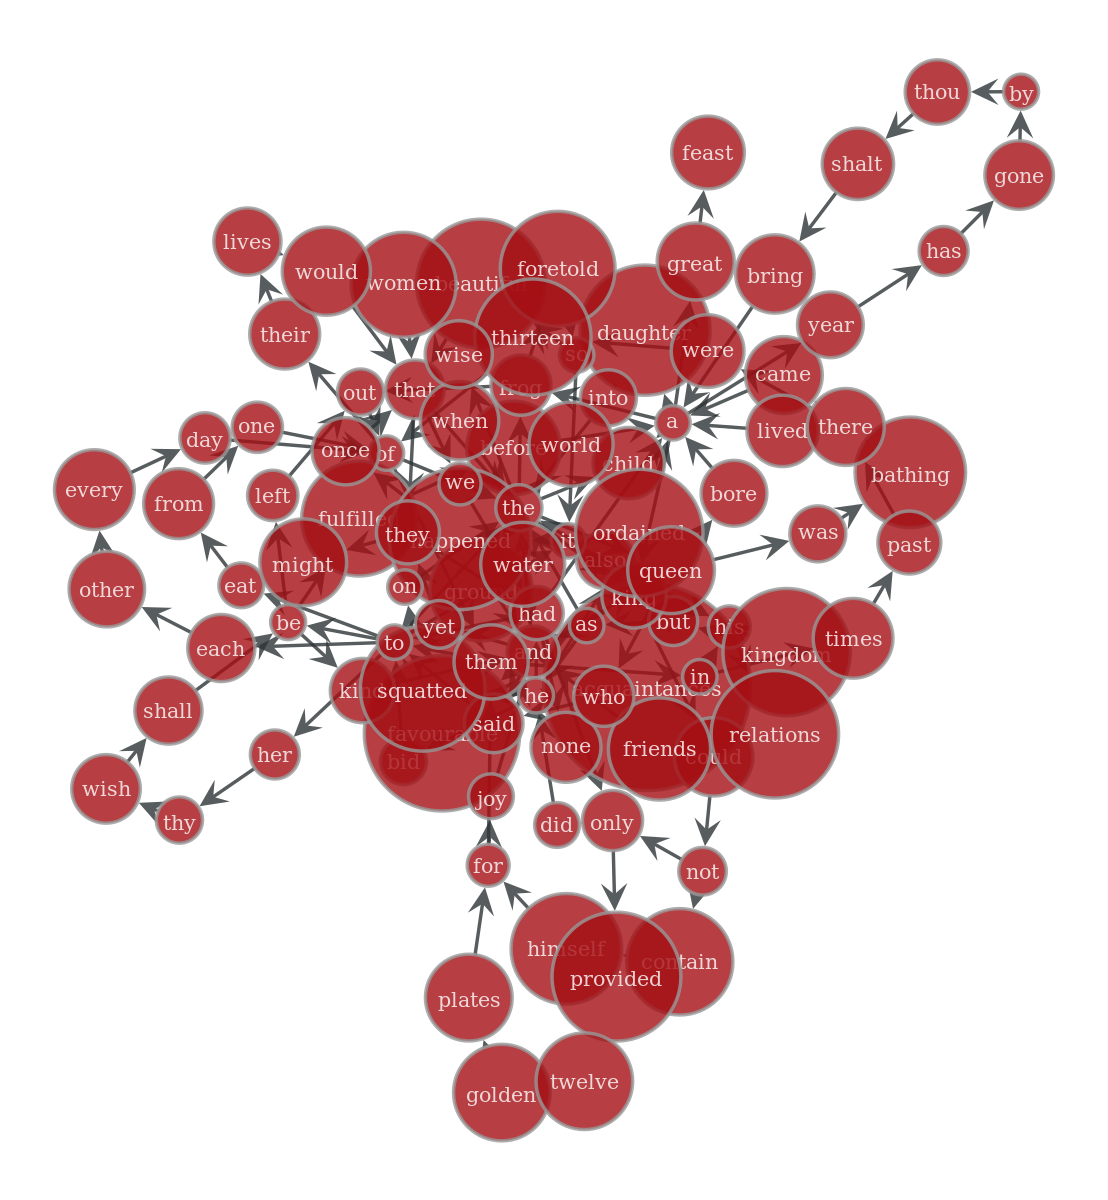
\includegraphics[scale=0.2]{englishwordgraph.png}
	\caption{Graph generated based on an extract of the story "Sleeping Beauty" with each unique word labelling each vertex.}
	\label{fig:engword}
\end{subfigure}
\hfill
\begin{subfigure}{.45\textwidth}
	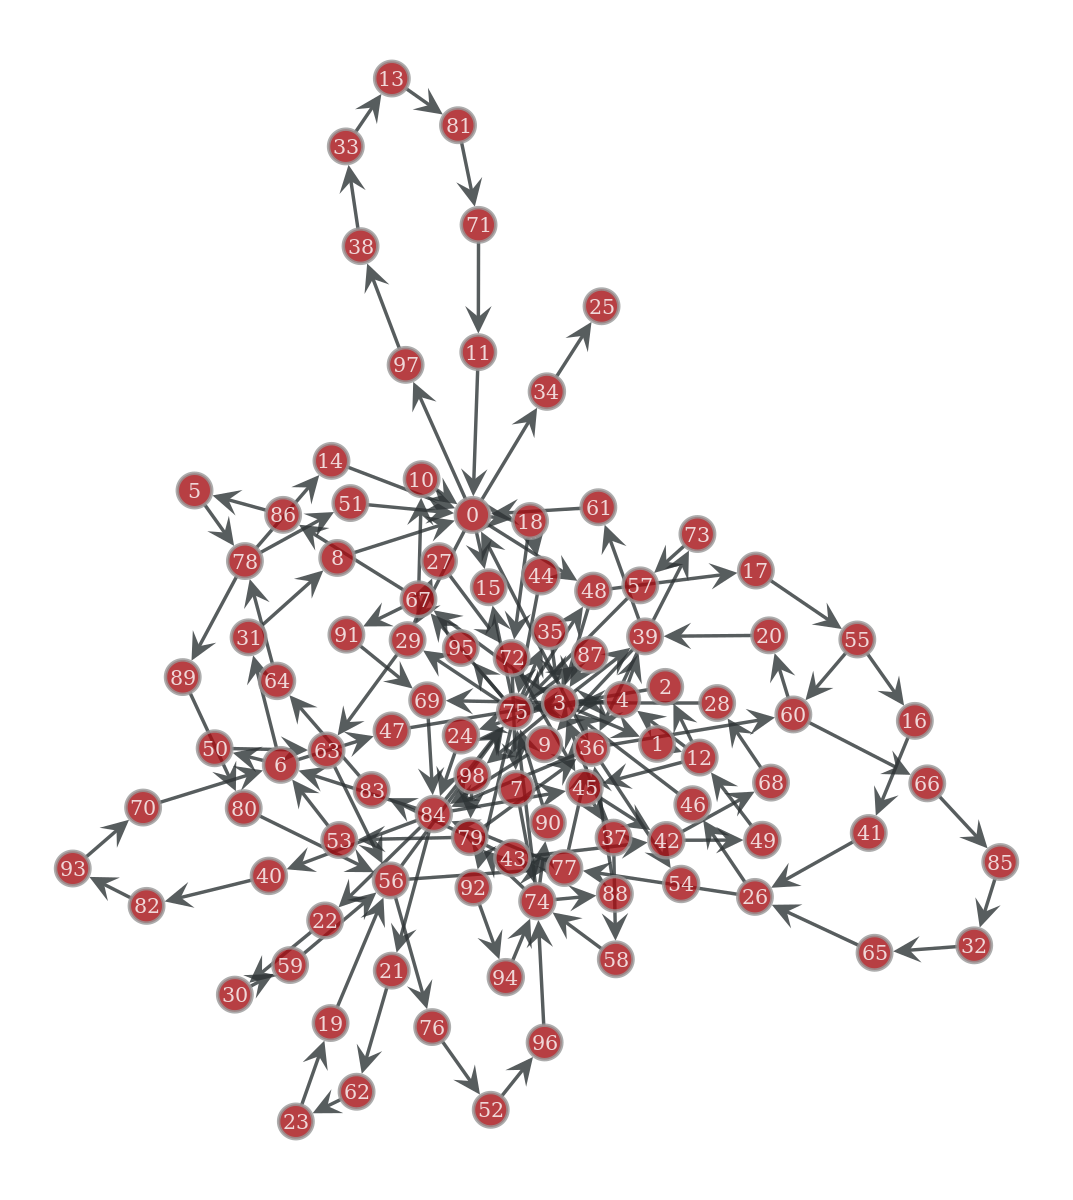
\includegraphics[scale=0.2]{englishnumbergraph.png}
	\caption{Same graph as the word graph for the English version of "Sleeping Beauty" but with numerical labelling rather than the corresponding words. The numbers are labelled in order of the unique words in alphabetical order which is also shown in the table later on.}
	\label{fig:engnum}
\end{subfigure}
\end{figure}

As done in the Early Experimentations of the karate club dataset, we calculate the values of the various graph properties explained in Chapter 2. These are graph properties such as local clustering coefficient, betweenness centrality, closeness centrality, trophic levels and page rank. Values are organised into their correpsonding columns and presented as a table as shown in Table \ref{table:english} which includes the number of appearanes the word has denoted as count and the relative vertex number in the numbered english graph.

\begin{table}[H]
	\centering
	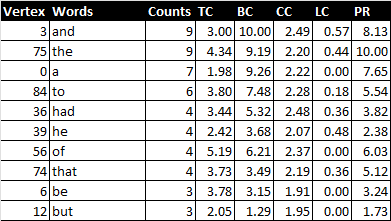
\includegraphics[scale=1]{englishtabletop10.png}
	\caption{The initial graph based on the karate club dataset pre-existing within the library that was generated through the python program. Contains 34 clubs and their connections to one another with no important meaning with the positions of the vertices.}
	\label{table:english}
\end{table}


\begin{figure}[H]
	\centering
	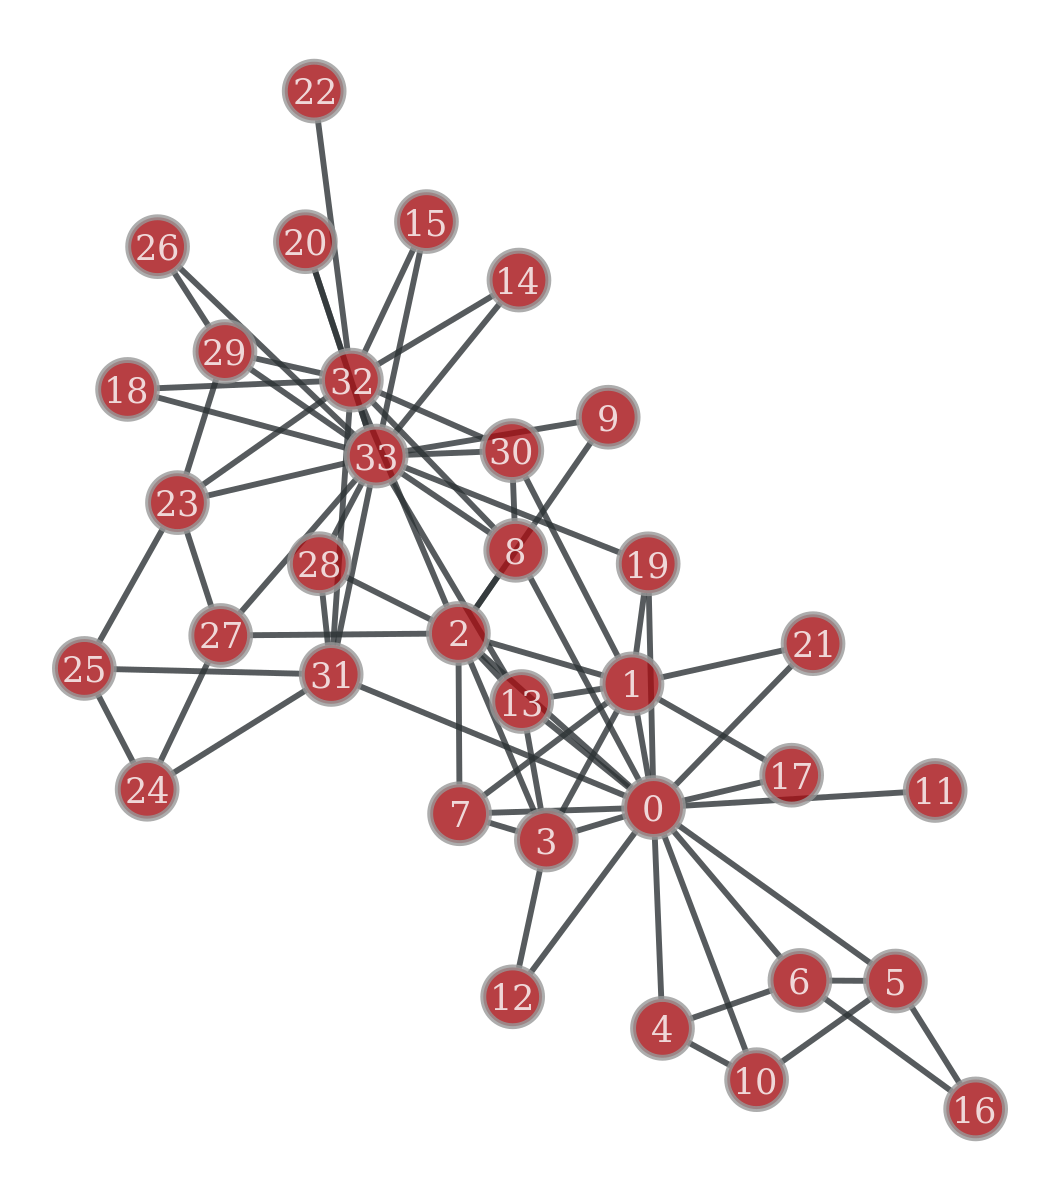
\includegraphics[scale=0.20]{karate.png}
	\caption{The initial graph based on the karate club dataset pre-existing within the library that was generated through the python program. Contains 34 clubs and their connections to one another with no important meaning with the positions of the vertices.}
	\label{fig:karate}
\end{figure}
